\documentclass[beamer,dvipsnames]{standalone}

\usepackage{tikz}
\usetikzlibrary{arrows}
\usetikzlibrary{positioning}
%\usetikzlibrary{positioning,decorations.pathreplacing,fit}
\usetikzlibrary{decorations.markings,arrows.meta}

\usepackage{bm}

\providecommand{\Key}{\textcolor{Orange}{K}}
\providecommand{\key}{\textcolor{blue}{sk}}

\providecommand{\dlog}[2]{\textcolor{#1}{#2}}
\providecommand{\ua}[1]{\dlog{red}{#1}}
\providecommand{\ub}[1]{\dlog{blue}{#1}}
\providecommand{\uc}[1]{\dlog{Plum}{#1}}
\providecommand{\ud}[1]{\dlog{OliveGreen}{#1}}

\begin{document}

\begin{standaloneframe}

\resizebox{1\textwidth}{!}{

\begin{tikzpicture}[
	>=triangle 60,
   	every path/.style={
   		thick
   	},
	arrow double line/.style={
		double distance = 20pt,
   		shorten <= 11, 	
   		shorten >= 11,
%   		very thick,
	    postaction = {
    		draw = white,
	 	    line width = 20pt,
	 	    shorten <=-.1pt,
	 	    shorten >=-.1pt,	
	    },
	    postaction = {
	    	decorate, 
	    	decoration = {
	    		markings, 
	    		mark=at position 0 with {
	    			\arrow[xshift=14.7pt]{Straight Barb[reversed,length=13pt 1]}
	    		},
	    		mark = at position 1 with {
   	    			\arrow[xshift=0pt]{Straight Barb[length=13pt 1]}
   	    		}
	    	}
	    }
	},
%	every node/.style={
%		font=\bfseries\boldmath
%	},
]

	\node (A) {};
	\node[right=3cm of A] (B) {};
	\node[right=3cm of B] (C) {};
	\node[right=6cm of C] (D) {};
	
	\node[above = 0 of A] {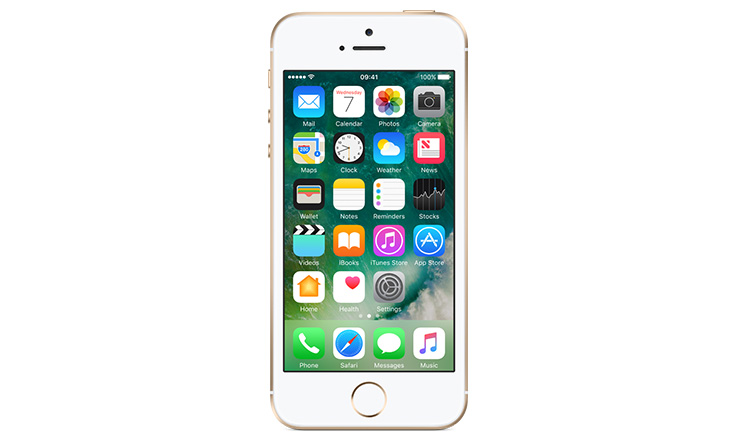
\includegraphics[width=0.25\textwidth]{cellphone}};
	\node[above = 0 of B] {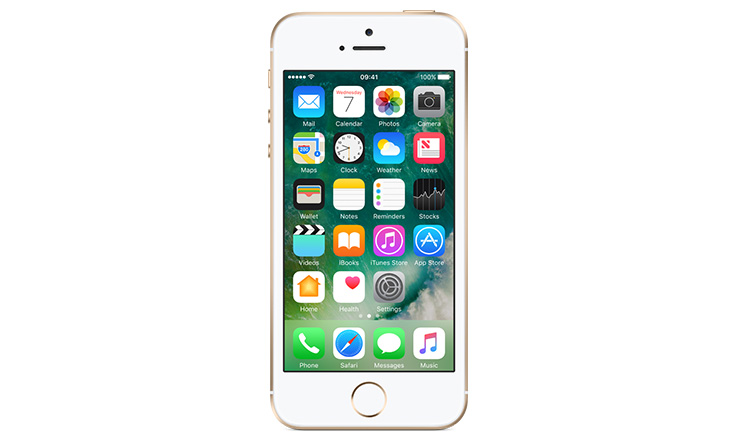
\includegraphics[width=0.25\textwidth]{cellphone}};
	\node[above = 0 of C] {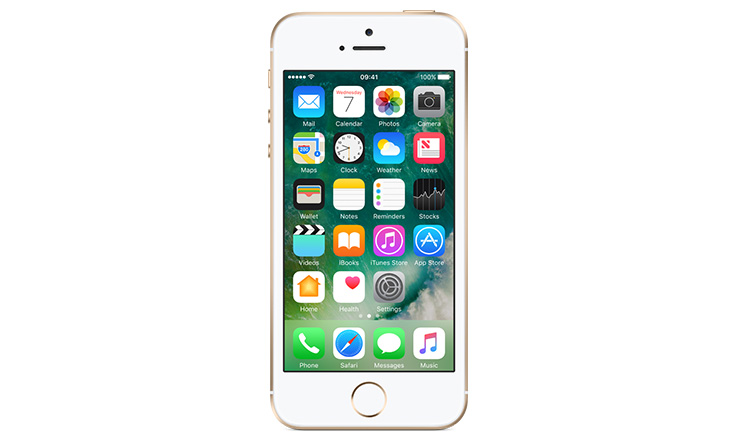
\includegraphics[width=0.25\textwidth]{cellphone}};
	\node[above = 0 of D] {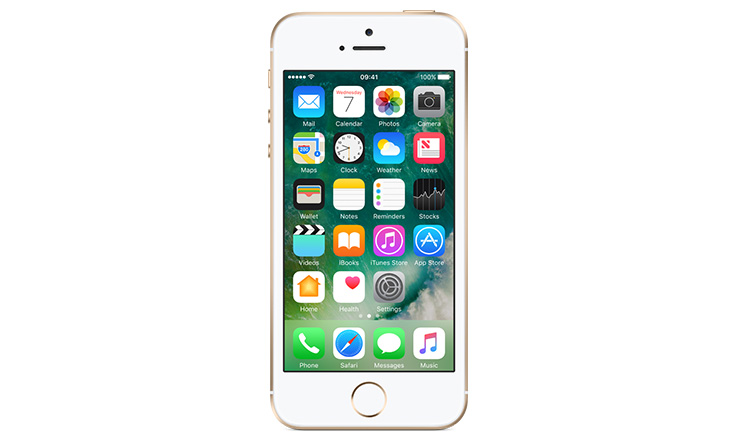
\includegraphics[width=0.25\textwidth]{cellphone}};
	
	
	\newcommand*{\MsgSpace}{0.8}
	\foreach \i in {1, ..., 9} {
		\node[below = \i * \MsgSpace of A,inner xsep=10pt] (a\i) {};
		\node[below = \i * \MsgSpace of B,inner xsep=10pt] (b\i) {};
		\node[below = \i * \MsgSpace of C,inner xsep=10pt] (c\i) {};
		\node[below = \i * \MsgSpace of D,inner xsep=10pt] (d\i) {};
	}
	
	


	\uncover<+-+(1)>{
		\draw[arrow double line,blue] (a1.east) -- node (KE) {Key exchange} (d1.west);
		\node at (a1) {$\key$};
		\node at (d1) {$\key$};
		\draw[arrow double line,Plum] (b3.east) -- node (KE) {Key exchange} (d3.west);
		\node[Plum] at (b3) {$sk$};
		\node[Plum] at (d3) {$sk$};
		\draw[arrow double line,OliveGreen] (c5.east) -- node (KE) {Key exchange} (d5.west);
		\node[OliveGreen] at (c5) {$sk$};
		\node[OliveGreen] at (d5) {$sk$};
	}

	\uncover<+-+>{
		\node[above right =-0.6cm and -5pt of d6, align=left] {$\ua{\mathsf{GK}} \gets \lbrace 0,1 \rbrace^{256}$};
		\draw[<-] (a7.east) -- node[above] {$\mathsf{Enc}(\ub{sk},\ua{\mathsf{GK}})$} (d7.west);
		\draw[<-] (b8.east) -- node[above] {$\mathsf{Enc}(\uc{sk},\ua{\mathsf{GK}})$} (d8.west);
		\draw[<-] (c9.east) -- node[above] {$\mathsf{Enc}(\ud{sk},\ua{\mathsf{GK}})$} (d9.west);
	}

	\uncover<+->{
		\node[above right= 1.2 and 0.5 of A] {$\ua{\mathsf{GK}}$};
		\node[above right= 1.2 and 0.5 of B] {$\ua{\mathsf{GK}}$};
		\node[above right= 1.2 and 0.5 of C] {$\ua{\mathsf{GK}}$};
		\node[above right= 0.9 and 0.2 of D] {$\ua{\mathsf{GK}}$};
	}

	\uncover<+->{
		\draw[<-] (a1.north east) -- node[above,pos=0.3] {$\mathsf{Enc}(\ua{\mathsf{GK}}, M)$} (d1.north west);
		\draw[<-] (b2.east) -- node[above,sloped, pos=0.3] {$\mathsf{Enc}(\ua{\mathsf{GK}}, M)$} ([yshift=-2pt]d1.south west);
		\draw[<-] (c3.east) -- node[above,sloped, pos=0.45] {$\mathsf{Enc}(\ua{\mathsf{GK}}, M)$} ([yshift=1pt]d2.north west);
	}


	
\end{tikzpicture}

}

\end{standaloneframe}

\end{document}